\documentclass{beamer}

\usepackage[spanish]{babel}
\decimalpoint
\usepackage[utf8]{inputenc}
\usepackage{ragged2e} % este paquete es para justificar.
\justifying
\usepackage{booktabs}
\usepackage{verbatim}
\usepackage{amsmath}
\usepackage{bm} % bold font greek letters. Use \boldsymbol{ }  and \pmb
\usepackage{xfrac} % for slanted fractions   \sfrac{}{}
\usepackage{nicefrac} % for small fractions in text or math mode   \nicefrac{}{}
%\usepackage{blkarray} % for block arrays, useful for markov chains. Error with Metropolis Beamer Theme
\usepackage{hhline} % hlines  but interacts with vertical lines
\usepackage{multirow}
\usepackage{pgfpages} % for handouts
\usepackage{graphicx} % for graphics and grapics path
%
\usepackage{import} 
%
%\pgfpagesuselayout{4 on 1}[letterpaper,landscape]
\usepackage[font=scriptsize,labelfont=bf,justification=centerlast,format=hang]{caption} %To change the appearance of captions
% tikz
\usepackage{tikz} % for draw
\usetikzlibrary{automata,arrows,positioning,calc}
\graphicspath{{figs/}}


\definecolor{tealsection}{RGB}{50,90,90}
\hypersetup{colorlinks=true,
  urlcolor=red,
  linkcolor=tealsection}

\usepackage[T1]{fontenc}
\usepackage{listings}

\definecolor{keywords}{RGB}{255,0,90}
\definecolor{comments}{RGB}{60,179,113}
\lstset{
  language=Python,
  basicstyle=\footnotesize\fontfamily{fvm}\selectfont,
  keywordstyle=\color{keywords},
  commentstyle=\color{comments}\emph
}

% ========================================
\newenvironment<>{exercise}[1]
{
\setbeamercolor{block title}{fg=white,bg=orange!45!black}
\begin{block}#2{Ejercicio #1}\justifying
}
{%
\end{block}
}%
% ========================================
\newenvironment<>{solution}[1]
{
\setbeamercolor{block title}{fg=white,bg=orange!65!black}
\begin{block}#2{Ejercicio #1 (Solución)}\justifying
}
{
\end{block}
}
% ========================================
\newenvironment<>{example}[1]
{
\setbeamercolor{block title}{fg=white,bg=green!65!black}
\begin{block}#2{Ejemplo #1}\justifying
}
% content
{
\end{block}
}
% ========================================
\newenvironment<>{frameExample}[2]
{
\setbeamercolor{frametitle}{fg=white,bg=green!60!blue}
\begin{frame} \justifying
  \frametitle{Ejemplo: #1}
  \framesubtitle{\insertsubsectionhead #2}
  
}
% content
{
\end{frame}
}
% ========================================
\newenvironment<>{framecode}[1][] % for coding
{
\setbeamercolor{frametitle}{fg=white,bg=black!85}
\begin{frame}[environment=fr,#1]
\frametitle{}
\framesubtitle{}
}%
{
\end{frame}
}
% ========================================
\newenvironment<>{frameact}[1] % For Activities
{
%\usebackgroundtemplate{\includegraphics[scale=0.3]{blackboard-logo.png}}
\setbeamercolor{frametitle}{fg=white,bg=red!60!black}
\begin{frame}\justifying
  \frametitle{Actividad: #1}
  \framesubtitle{}
%{\centering \includegraphics[scale=0.5]{BlackBoardSymbol.png}\par}
%\vspace{5mm}

}
{
\end{frame}
}
% ========================================
%\graphicspath{}
\usetheme[%
sectionpage=progressbar,
numbering=none,
progressbar=frametitle%
]{metropolis}
%\usetheme{Boadilla}

\title{Modelos Matemáticos}
\subtitle{Asignatura: Optimización de Sistemas} % 6 hours. 2 sessions


\institute{UNIVERSIDAD ANÁHUAC MÉXICO}
\author{Rafael Torres Escobar, Ph.D.}
\date[Anáhuac México]{}


 \AtBeginSection[] % Do nothing for \section* %
{
\begin{frame}<beamer> 
  \frametitle{Agenda}
  \tableofcontents[currentsection] 
\end{frame}
}


%%%%%%%%%%%%%%%%%%%%%%%%%%%%%%

\begin{document}

\begin{frame}
  \maketitle
\end{frame}


     \begin{frame}{Agenda}
   \tableofcontents
 \end{frame}


\section{Investigación de Operaciones}
\label{sec:operations-research}

\begin{frame}{Hitos Históricos en Investigación de Operaciones}
  Antes, Durante y Después de la Segunda Guerra Mundial

  {\centering
    
\includegraphics[scale=0.5]{ww2_01}
    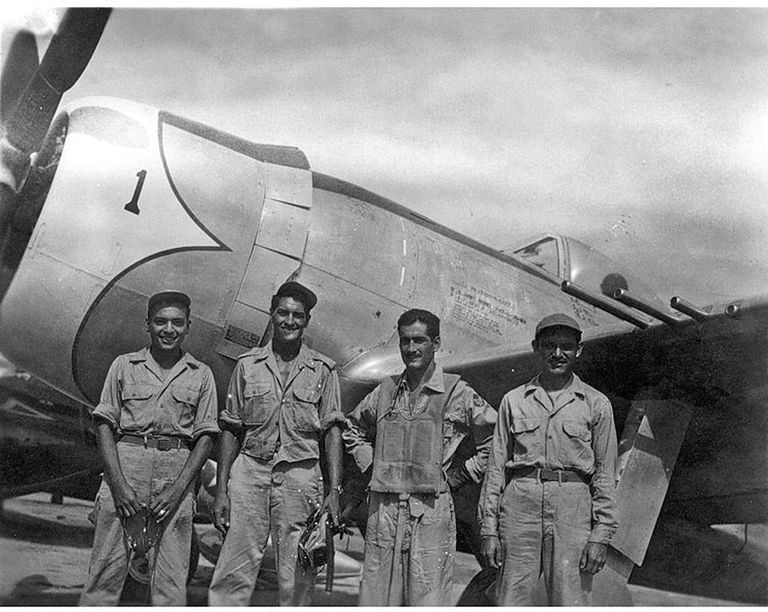
\includegraphics[scale=0.2]{ww2_02}
  \par}
\end{frame}

\begin{frame}{Desarrollo de la Investigación de Operaciones}
 \label{slide:or-dates}
  \begin{itemize} \justifying \parskip3mm
  \item<only@1> 1855. \href{https://en.wikipedia.org/wiki/Frederick_Winslow_Taylor}{Frederick W. Taylor}
  \item<only@1> 1884.  \href{https://en.wikipedia.org/wiki/Henry_Gantt}{Henry Gantt}
  \item<only@1> 1915. \href{https://en.wikipedia.org/wiki/Ford_Whitman_Harris}{Ford Whitman Harris}
  \item<only@1> 1917. \href{https://en.wikipedia.org/wiki/Agner_Krarup_Erlang}{A.K. Erlang}
  \item<only@1> 1930. \href{https://en.wikipedia.org/wiki/Horace_Clifford_Levinson}{Horace Clifford Levinson}
  \item<only@2> 1940. \href{https://www.informs.org/Explore/History-of-O.R.-Excellence/Biographical-Profiles/Blackett-Patrick-M.-S}{Patrick Maynard Stuart Blackett}  
    \item<only@2> 1947. \href{https://en.wikipedia.org/wiki/George_Dantzig}{George Dantzig}
    \item<only@2> 1950. \href{https://en.wikipedia.org/wiki/Ralph_E._Gomory}{Ralph E. Gomory}
  \item<only@2> \href{https://www.youtube.com/watch?v=ILWbaWrjgU4}{Historia de la IO} 
  \end{itemize}
\end{frame}


\begin{frame}{Características de la I.O.}
  \begin{enumerate} \justifying \parskip3mm
  \item Orientada a Sistemas
  \item Equipos interdisciplinarios
  \item Método Científico
  \item Nuevos Problemas
  \item Mejorar la calidad de las decisiones
  \item Tecnología
  \item Soluciones cuantitativas
  \item Factor humano
  \end{enumerate}
\end{frame}

\begin{frame}{Método Científico}
  \begin{enumerate} \justifying \parskip3mm
  \item Juicio
  \item Investigación
  \item Acción
  \end{enumerate}

  {\centering
      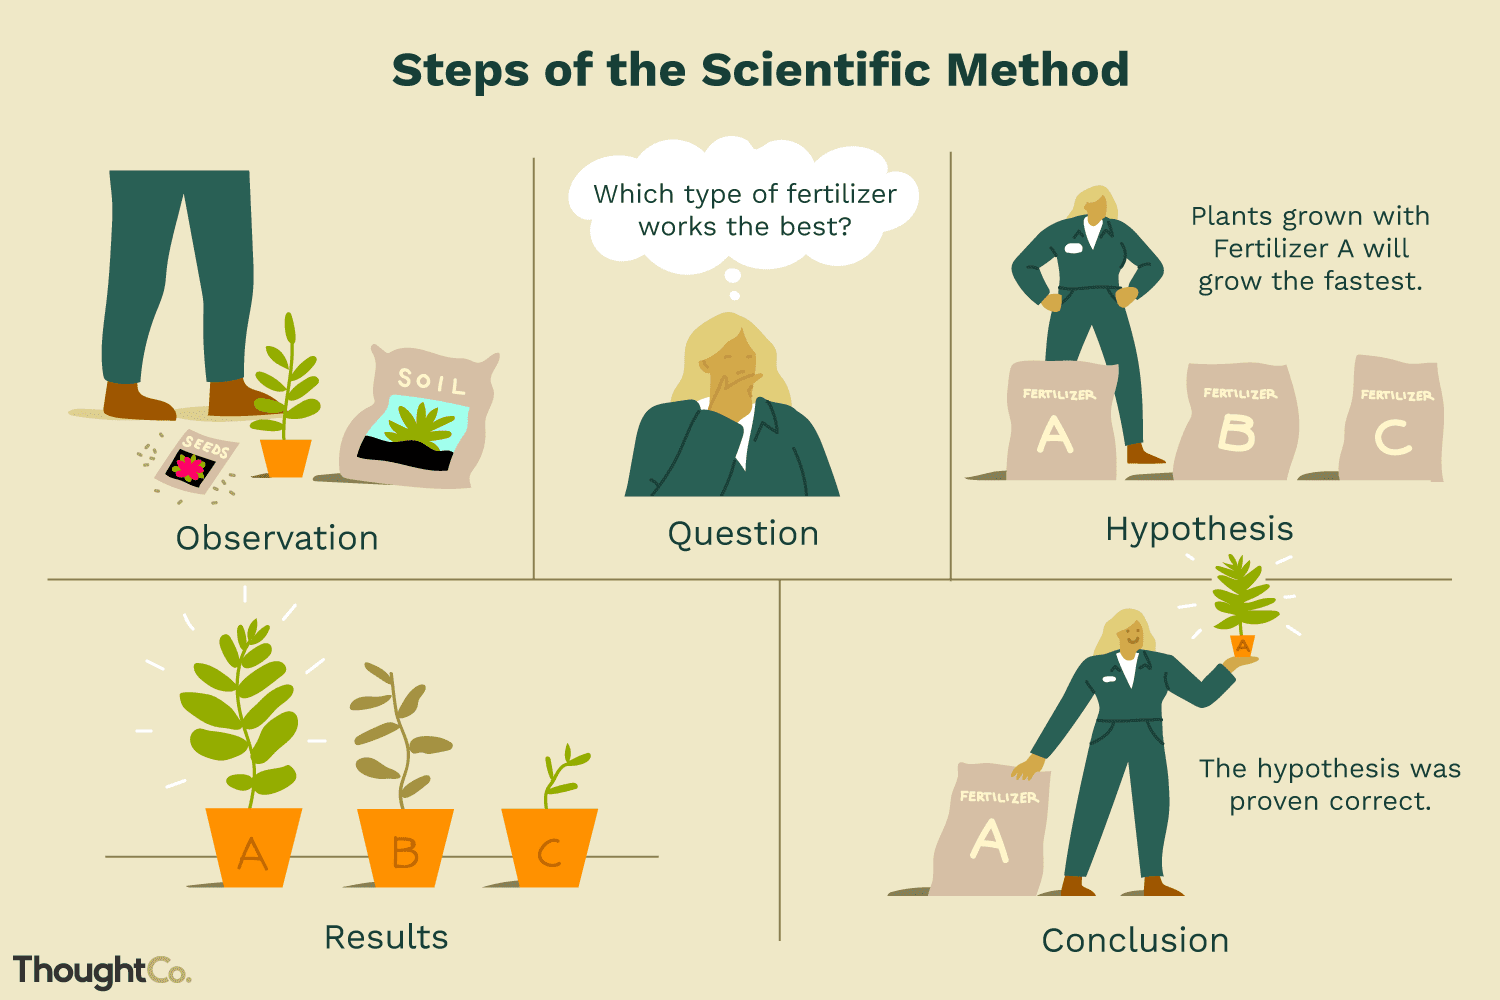
\includegraphics[scale=0.15]{scientific-method}
  \par}
\end{frame}

\begin{frame}{I.O. en Administración}
  \begin{columns}
    \column{0.5\textwidth}
\begin{itemize} \justifying \parskip3mm
  \item<only@1> Distribución
  \item<only@1> Planeación de la producción
  \item<only@1> Adquisiciones
  \item<only@1> Marketing
  \item<only@1> Finanzas
  \item<only@1> Investigación y Desarrollo
  \item<only@2>  Flujo de Efectivo
  \item<only@2> Control de Inventarios
  \item<only@2> Simulación
  \item<only@2> Presupuesto  
  \end{itemize}
  
  \column{0.5\textwidth}
  {\centering
    \includegraphics<1>[scale=0.5]{factory}
    \includegraphics<1>[scale=0.5]{logistics}
        \includegraphics<2>[scale=0.4]{logistics02}
  \par}
  \end{columns}
\end{frame}


\begin{frame}{Técnicas de I.O.}
  
  \begin{columns}
    \column{0.5\textwidth}
    \begin{enumerate} \justifying \parskip2mm
\item Programación Lineal.
\item Programación Dinámica.
\item Control de Inventarios.
\item Líneas de Espera.
\item Teoría de la Decisión.
\item Redes. CPM y PERT
\item Simulación.
\item Reemplazo
\end{enumerate}

\column{0.5\textwidth}
{\centering
  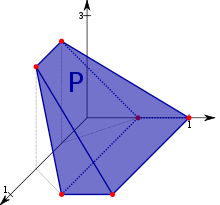
\includegraphics[scale=0.5]{polythope}
  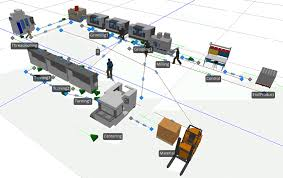
\includegraphics[scale=0.5]{simulation}
\par}
  \end{columns}
\end{frame}

\begin{frame}{Metodología}
  \begin{enumerate} \justifying \parskip3mm
  \item Formulación del Problema.
  \item Construcción del modelo.
  \item Solución.
  \item Verificación, validación. 
  \item Análisis de sensibilidad.
  \item Implementación.
  \end{enumerate}
\end{frame}


\begin{frameact}{Importancia de la  I.O.}
  En un documento Word o Google Docs escribe lo que se pide a continuación:

  \begin{itemize} \justifying  \parskip3mm
  \item Menciona en párrafos de 4 líneas como máximo las aportaciones que realizaron a la Investigación de Operaciones los siguientes científicos Blackett, Dantzig y Gomory. Usar un párrafo para cada personaje.   \hyperlink{slide:or-dates}{Dar click aquí}  para ver los links de cada biografía. % \href{https://www.youtube.com/watch?v=jg5IQ5Hf2G0}{Patrick Blackett. Draw my life (video)} que aparece en video del enlace.

  \item En tus propias palabras escribe una reflexión de máximo media cuartilla sobre el impacto que tiene la Investigación de Operaciones en nuestra vida a partir del video del \href{https://www.youtube.com/watch?v=sFWrmpXPVJw}{INFORMS Institute}
  \end{itemize}
\end{frameact}


%%% Local Variables:
%%% mode: latex
%%% TeX-master: "../slides"
%%% End:


\begin{frameact}{FedEx}
  Lea el artículo de referencia que describe todo el estudio de I.O. para FedEx. Enliste los diferentes beneficios financieros y no financieros que resultaron de este estudio. El artículo está disponible en el siguiente enlace: \href{https://drive.google.com/file/d/1b8VCLpjFeBWOssiuRRNjnjSkSGwoGaA9/view?usp=sharing}{“Absolutely, Positively Operations Research: The Federal Express Story”}
\end{frameact}


%%% Local Variables:
%%% mode: latex
%%% TeX-master: "../slides"
%%% End:


%%% Local Variables:
%%% mode: latex
%%% TeX-master: "slides"
%%% End:

\section{Modelos en Investigación de Operaciones}
\label{sec:taxonomy}


\begin{frame}{Clasificación de los Modelos}
  \begin{enumerate} \justifying \parskip3mm
  \item<only@1,2> Grado de abstracción.
  \item<only@1,3> Función.
  \item<only@1,4> Estructura.
  \item<only@1,5> Naturaleza del medio ambiente.
  \item<only@1,6> Generalidad.
  \item<only@1,7> Horizonte temporal.
  \end{enumerate}

  {\centering
    \includegraphics<2>[scale=0.15]{fig_mathmodel}
    \includegraphics<2>[scale=0.2]{fig_languagemodel}
    
    \includegraphics<3>[scale=0.2]{fig_descriptive}
    \includegraphics<3>[scale=0.3]{fig_predictive}
    \includegraphics<3>[scale=0.4]{fig_prescriptive}

    \includegraphics<4>[scale=0.04]{fig_iconic}
    \includegraphics<4>[scale=0.5]{fig_schematic}
    \includegraphics<4>[scale=0.2]{fig_mathematical}

    \includegraphics<5>[scale=0.5]{fig_deterministic}
    \includegraphics<5>[scale=0.5]{fig_probabilistic}

    \includegraphics<6>[scale=0.5]{fig_general}
    \includegraphics<6>[scale=0.5]{fig_specific}

    \includegraphics<7>[scale=0.5]{fig_static}
    \includegraphics<7>[scale=0.2]{fig_dynamic}
  \par}
\end{frame}




%%% Local Variables:
%%% mode: latex
%%% TeX-master: "slides"
%%% End:


\section{Estructura de los modelos matemáticos}
\label{sec:formulations}



\begin{frame}{Consideraciones en Un Modelo }
  \begin{enumerate} \justifying \parskip3mm
  \item Factibilidad
  \item Optimalidad
  \item Sensibilidad
  \item Implementación
  \end{enumerate}
\end{frame}

% Example with python
\begin{frameExample}{Maximizar Utilidad}{}
  \only<1>{%
  Una compañía se enfrenta a la demanda de un producto. La demanda es una función del precio y ambos, el precio $p$ y la cantidad $q$ los decide la compañía. Se sabe que la relación precio-cantidad es $p = 10 - 0.01q$, lo que significa que a partir de \$10 por unidad, cada aumento unitario de la demanda disminuye el precio que todos los clientes están dispuestos a pagar por el producto en 1 centavo. Cuesta \$5 fabricar una unidad, y los costos generales independientes de la cantidad ascienden a \$ 500. La compañía quiere maximizar ganancias.%
  }

  \begin{onlyenv}<2>
    \begin{align*}
    \text{Precio} & = 10 - 0.01q\\
    \text{Costo Variable} & = 5q \\
    \text{Costo Fijo} & = 500\\[3mm]
    \text{Ingresos} & = \text{Precio} * \text{Cantidad} = (10 - 0.01q)q\\
    \text{Costos} &= \text{Costo Variable} + \text{Costo Fijo}\\[5mm]
      \text{Ganancia} &=  \text{Ingresos} - \text{Costos}\\
                  & = (10 - 0.01q)q - (5q + 500)\\
      & = -0.01q^2 + 5q - 500\\
  \end{align*}
  \end{onlyenv}

  \begin{alertblock}<only@3>{Descargar Anaconda Python} \justifying
      Si aún no has descargado la \href{https://www.anaconda.com/products/individual}{Distribución Aconda Python}, puedes usar \href{https://colab.research.google.com/notebooks/intro.ipynb}{Google Colab} con una cuenta de Gmail.
    \end{alertblock}
    
\end{frameExample}


\begin{frame}[fragile]{Ejemplo. Uso de Python}

  
  \begin{lstlisting}
import numpy as np
from scipy.optimize import root, minimize
from matplotlib import pyplot as plt

q = np.linspace(100,400, 500)

# Parameters
p = 10
w = 0.01
# w = 0.005

var_cost = 5
# var_cost = 6

fix_cost = 500
# fix_cost = 500

  \end{lstlisting}
\end{frame}

\begin{frame}[fragile]{Python}

  \begin{lstlisting}
price = lambda a, b, q: a - b*q
    
def f(x, cost1=var_cost, cost2=fix_cost):
    return (price(p, w, x))*x - (cost1 * x + cost2)

P = f(q)
plt.plot(q, P)
plt.axhline(0, color='gray')
plt.show()
  \end{lstlisting}
\end{frame}

\begin{frame}[fragile]{Python. Encontrar Raíces}

  \begin{lstlisting}
sol = root(f, [100, 400])
print(f'Quantities {sol.x}')
print(f'Price1: {price(p, w, sol.x[0])}')
print(f'Price2: {price(p, w, sol.x[1])}')
  \end{lstlisting}
\end{frame}


\begin{frame}[fragile]{Python. Maximizar una función}

  \begin{lstlisting}
def f2(x):
    return -f(x)

max_result = minimize(f2, 300),
print(-max_result[0]['fun'])
print(max_result[0]['x'])
  \end{lstlisting}
\end{frame}


%%% Local Variables:
%%% mode: latex
%%% TeX-master: "../slides"
%%% End:


\begin{frame}{Estructura De Un Modelo Matemático}

Todos los modelos de IO, incluido el de Programación Lineal (PL), constan de tres componentes básicos.

  \begin{enumerate} \justifying 
  \item Los \alert{parámetros} o variables externas que no están bajo nuestro control.
  \item Las \alert{variables de decisión} que pretendemos determinar.
  \item El \alert{objetivo} (la meta) que necesitamos optimizar (maximizar o minimizar).
  \item Las \alert{restricciones} que la solución debe satisfacer.
  \end{enumerate}
   
\end{frame}


\section{Ejemplos de Modelado Matemático}
\label{sec:model-examples}


\begin{frameExample}{Reddy Mikks}{}
   % Ejemplo 2.1-1 (La compañía Reddy Mikks) Taha
  \only<1>{%
    Reddy Mikks produce pinturas para interiores y exteriores con dos materias primas, $M_1$ y $M_2$. La tabla siguiente proporciona los datos básicos del problema. Una encuesta de mercado indica que la demanda diaria de pintura para interiores no puede exceder la de pintura para exteriores en más de una tonelada. Asimismo, que la demanda diaria máxima de pintura para interiores es de dos toneladas. Reddy Mikks se propone determinar la (mejor) combinación óptima de pinturas para interiores y exteriores que maximice la utilidad diaria total.%
  }


  {\centering
  \includegraphics<1>[scale=0.6]{reddy-mikks_01}
  \par}
\end{frameExample}



%%% Local Variables:
%%% mode: latex
%%% TeX-master: "../slides"
%%% End:

\begin{frameact}{Reddy Mikks Formulations}{}
 Para el modelo de \hyperlink{example:reddy-mikks}{Reddy Mikks}, defina las siguientes restricciones y expréselas con un lado izquierdo lineal y un lado derecho constante

(a) La demanda diaria de pintura para interiores supera la de pintura para exteriores
por al menos una tonelada.

(b) El consumo diario de materia prima $M_2$ en toneladas es cuando mucho de 6 y por
lo menos de 3.

(c) La demanda de pintura para interiores no puede ser menor que la demanda de pintura para exteriores.

(d) La cantidad mínima de pintura que debe producirse tanto para interiores como para exteriores es de 3 toneladas.

(e) La proporción de pintura para interiores respecto de la producción total de pintura
para interiores y exteriores no debe exceder de 0.5

\end{frameact}


%%% Local Variables:
%%% mode: latex
%%% TeX-master: "../slides"
%%% End:


\begin{frameExample}{Producción}{}
  % EXAMPLE 2.6-1 (Production Allocation Problem} Gupta ebook
  Una empresa produce tres productos. Estos productos se procesan en tres máquinas diferentes. El tiempo requerido para fabricar una unidad de cada uno de los tres productos y la capacidad diaria de las tres máquinas se detallan en la tabla a continuación.

  {\centering
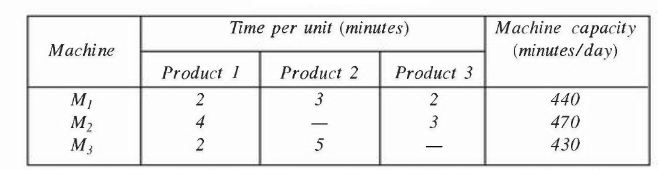
\includegraphics[scale=0.5]{example_allocation_gupta}
\par}

   Se requiere determinar la cantidad diaria de unidades que se fabricarán para cada producto. El beneficio por unidad para el producto 1, 2 y 3 es de \$ 4, \$ 3 y \$ 6 respectivamente. Se supone que todas las cantidades producidas se consumen en el mercado. Formule el modelo matemático (L.P.) que maximizará la ganancia diaria.
\end{frameExample}



%%% Local Variables:
%%% mode: latex
%%% TeX-master: "../slides"
%%% End:

\begin{frameExample}{Dieta}{}
  % EXAMPLE 2.6-2 {Diet Problem} Gupta
  La persona quiere decidir los componentes de una dieta que cumpla con sus requerimientos diarios de proteínas, grasas y carbohidratos al costo mínimo. La elección debe hacerse a partir de cuatro tipos diferentes de alimentos. Los rendimientos por unidad de estos alimentos se dan en la tabla siguiente. Formule un modelo de programación lineal para el problema.
  
  {\centering
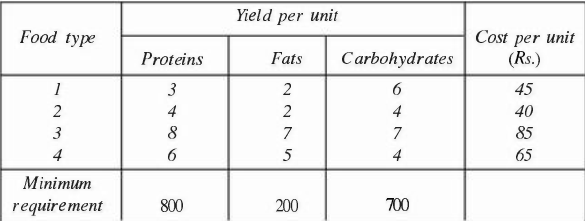
\includegraphics[scale=0.5]{example_diet_gupta}
\par}

  
\end{frameExample}



%%% Local Variables:
%%% mode: latex
%%% TeX-master: "../slides"
%%% End:

\begin{frameExample}{Mezcla}{}
  % EXAMPLE 2.6-3 (Blending Problem) 
  \only<1>{%
    Una empresa produce una aleación que tiene las siguientes especificaciones:

\begin{enumerate}[i)]  \justifying
\item  gravedad específica $\leq$ O. 98,
\item  cromo $\geq$ 8\%,
\item  punto de fusión $\geq$ 450°C.
\end{enumerate}

Las materias primas A, B y C que tienen las propiedades que se muestran en la tabla pueden usarse para hacer la aleación.%
}

  {\centering
\includegraphics<1,2>[scale=0.5]{example_blending_gupta}
\par}

\only<2>{Los costos de las diversas materias primas por tonelada son: \$ 90 para A, \$ 280 para B y \$ 40 para C. Formule el modelo L.P. para encontrar las proporciones en las que se utilizarán A, B y C para obtener una aleación de las propiedades deseadas, mientras que el costo de las materias primas es mínimo.}
    
\end{frameExample}



%%% Local Variables:
%%% mode: latex
%%% TeX-master: "../slides"
%%% End:

\begin{frameExample}{Seleccion de Medios}{}
  % LE 2.6-4 (Advertising Media Selection Problem) 

  \only<1>{%
  Una empresa de publicidad desea planificar su estrategia publicitaria en tres medios diferentes de televisión, radio y revistas. El objetivo de la publicidad es llegar al mayor número posible de clientes posibles. Se han obtenido los siguientes datos de una encuesta de mercado:%
  }

    {\centering
\includegraphics<1,2>[scale=0.5]{example_selection-media_gupta}
\par}

\only<2>{%
La compañía quiere gastar no más de \$ 450,000 en publicidad. Los siguientes son los requisitos adicionales que deben cumplirse:
\begin{enumerate}[i)] \justifying
\item  se producen al menos 1 millón de exposiciones entre clientes femeninas,
\item  la publicidad en revistas se limitará a \$ 150,000
\item  se deben comprar al menos 3 unidades publicitarias en la revista I y 2 unidades en la revista
\item  el número de unidades publicitarias en televisión y radio debe ser 5 y 10 cada uno.
\end{enumerate}

Formular un modelo L.P. para el problema.%
}
    
\end{frameExample}



%%% Local Variables:
%%% mode: latex
%%% TeX-master: "../slides"
%%% End:

\begin{frameExample}{Inspección}{}
  % EXAMPLE 2.6-5 {lnspection Problem} Gupta
Una empresa tiene dos grados de inspectores, I y II para llevar a cabo la inspección de control de calidad. Se deben inspeccionar al menos 1,500 piezas en un día de 8 horas. El inspector de grado I puede verificar 20 piezas en una hora con una precisión del 96\%. Grado II el inspector verifica 14 piezas por hora con un precisión del 92\%. Los salarios del inspector de grado I son \$ 5 por hora, mientras que los de grado II inspector son \$ 4 por hora. Cualquier error cometido por un inspector cuesta \$ 3 a la empresa. Si hay, en total, 10 grado I
inspectores y 15 inspectores de grado II en la empresa, encuentre la asignación óptima de inspectores que minimiza el costo diario de inspección.
    
\end{frameExample}



%%% Local Variables:
%%% mode: latex
%%% TeX-master: "../slides"
%%% End:

\begin{frameExample}{Mezcla de Productos}{}
  % EXAMPLE 2.6-6 (Product Mix Problem) Gupta
Una compañía química produce dos productos, $X$ e $Y$. Cada unidad de producto $X$ requiere 3 horas en operación I y 4 horas en operación II, mientras que cada unidad de producto $Y$ requiere 4 horas en operación I y 5 horas en operación II. El tiempo total disponible para las operaciones I y II es 20 horas y 26 horas respectivamente. La producción de cada unidad de producto $Y$ también da como resultado dos unidades de un subproducto $Z$ sin costo adicional. El producto $X$ se vende con una ganancia de \$ 10 / unidad, mientras que $Y$ se vende con una ganancia de \$ 20 / unidad. El subproducto $Z$ aporta un beneficio unitario de \$ 6 si se vende; en caso de que no se pueda vender, el costo de destrucción es de \$ 4 / unidad. Los pronósticos indican que no se pueden vender más de 5 unidades de $Z$. Formule el modelo L.P. para determinar las cantidades de $X$ e $Y$ que se producirán, teniendo en cuenta $Z$, de modo que la ganancia obtenida sea máxima.
    
\end{frameExample}



%%% Local Variables:
%%% mode: latex
%%% TeX-master: "../slides"
%%% End:

\begin{frameExample}{Mezcla de Productos (Fracciones)}{}
  % EXAMPLE 2.6-7 (Product Mix Problem) Gupta
Una empresa fabrica tres productos A, B y C. El tiempo para fabricar el producto A es el doble que para B y tres veces para C y si toda la mano de obra se dedica a la fabricación del producto A, se pueden producir 1,600 unidades de este producto. Estos productos deben producirse en una proporción de 3: 4: 5. Hay demanda de al menos 300, 250 y 200 unidades de productos A, B y C y el beneficio obtenido por unidad es de \$ 90, \$ 40 y \$ 30 respectivamente. Formule el problema como un problema de programación lineal.

{\centering
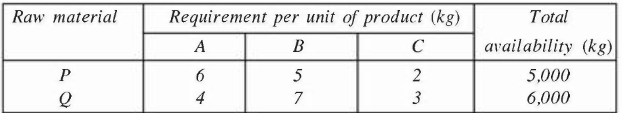
\includegraphics[scale=0.5]{example_product-mix02_gupta}
\par}

\end{frameExample}



%%% Local Variables:
%%% mode: latex
%%% TeX-master: "../slides"
%%% End:

\begin{frameExample}{Corte de Papel}{}
  % EXAMPLE 2.6-8 (Trim Loss Problem} 
  \only<1>{%
Una fábrica de papel produce rollos de papel utilizados para hacer cajas registradoras. Cada rollo de papel tiene una longitud de 100 m y se puede utilizar en anchos de 3, 4, 6 y 10 cm. El proceso de producción de la compañía da como resultado rollos de 24 cm de ancho. Por lo tanto, la empresa debe cortar su rollo de 24 cm al ancho deseado. Tiene seis alternativas básicas de corte de la siguiente manera:%
  }

  \begin{onlyenv}<1>
      {\centering
    \scalebox{0.7}{%
      \begin{tabular}{cccccc}
        \toprule
        Alternativas&\multicolumn{4}{c}{Ancho de los}&\\
        de corte&\multicolumn{4}{c}{rollos (cm)}&Desperdicio (cm)\\
        \cmidrule{2-5}
                    &3&4&6&10&\\
        \midrule[0.4pt]
        1&4&3&--&--&--\\
        2&--&3&2&--&--\\
        3&1&1&1&1&1\\
        4&--&--&2&1&2\\
        5&--&4&1&--&2\\
        6&3&2&1&--&1\\
        \bottomrule
      \end{tabular}
    }% \scalebox
% \includegraphics<1>[scale=0.5]{example_trim-loss_gupta}
\par}
  \end{onlyenv}

\only<2>{%
  La demanda mínima para los cuatro rollos es la siguiente:
  
{\centering
  \scalebox{0.8}{%
  \begin{tabular}{cr}
    \toprule
    Ancho del rollo (cm) & Demanda\\
     \midrule
    2 & 2,000 \\
    4 &3,600 \\
    6 &1,600 \\
    10 &500\\
    \bottomrule
  \end{tabular}
  }
  \par}

La fábrica de papel desea minimizar el desperdicio resultante del recorte al tamaño. Formule el modelo L.P.%
}

\end{frameExample}



%%% Local Variables:
%%% mode: latex
%%% TeX-master: "../slides"
%%% End:

\begin{frameExample}{Planeación de la Producción}{}
  % EXAMPLE 2.6-9 (Production Planning Problem) 
Una fábrica elabora un producto cuya unidad consta de 5 unidades de la parte A y 4 unidades de la parte B. Las dos partes A y B requieren diferentes materias primas, de las cuales están disponibles 120 unidades y 240 unidades respectivamente. Estas piezas pueden fabricarse por tres métodos diferentes. Los requisitos de materia prima por producción y el número de unidades para cada parte producida se detallan a continuación. Formule el modelo L.P. para determinar el número de corridas de producción para cada método a fin de maximizar el número total de unidades completas del producto final.

{\centering
%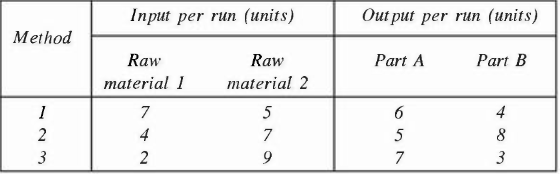
\includegraphics[scale=0.5]{example_production-planning_gupta}
  \scalebox{0.7}{%
    \begin{tabular}{ccccc}
      \toprule
  &\multicolumn{2}{c}{Entrada Por Corrida (unidades)}&\multicolumn{2}{c}{Salidas Por Corrida (unidades)}\\
  \cmidrule{2-5}
  Método&Materia & Materia & Parte&Parte \\
        &prima 1& prima 2&A&B\\
  \midrule
  1&7 &5 &6& 4\\
  2&4&7&5&8\\
  3&2&9&7&3\\
  \bottomrule
\end{tabular}
  } % \scalebox
\par}
\end{frameExample}

\begin{frameExample}{Planeación de la Producción}{}
  La función objetivo a maximizar es  \[ Z = \min \left(  \frac{6x_1 + 5x_2 + 7x_3}{5}, \frac{4x_1 + 8x_2 + 3x_3}{4}\right ) \]
  Las restricciones de disponibilidad de materias primas son:
  \begin{flalign*}
    7x_1 + 4x_2 +2x_3 &\leq 120\\
    5x_1 + 7x_2 +9x_3 &\leq 240\\
  \end{flalign*}
  La formulación anterior viola las propiedades de un programa lineal porque el objetivo es una función no lineal. El modelo se puede transformar a su versión equivalente lineal de la siguiente manera. 
  \[ y =  \min \left(  \frac{6x_1 + 5x_2 + 7x_3}{5}, \frac{4x_1 + 8x_2 + 3x_3}{4}\right )\]
  
\end{frameExample}

\begin{frameExample}{Planeación de la Producción}{}
  Tenemos entonces que
  \begin{flalign*}
    \frac{6x_1 + 5x_2 + 7x_3}{5} & \geq y\\
    \frac{4x_1 + 8x_2 + 3x_3}{4} & \geq y
  \end{flalign*}

  Por lo que el modelo matemático es:
\[ \max Z = y \]
sujeto a (s.t.)
  \begin{columns}[t]
    \column{0.4\textwidth}
\begin{flalign*}
    7x_1 + 4x_2 + 2x_3 & \leq 120\\
    5x_1 + 7x_2 + 9x_3 & \leq 240\\
  \end{flalign*}
  \column{0.4\textwidth}
    \begin{flalign*}
    6x_1 + 5x_2 + 7x_3 - 5y & \geq 0\\
    4x_1 + 8x_2 + 3x_3 - 4y & \geq 0\\
  \end{flalign*}
  \end{columns}
$x_1, x_2, x_3, y   \geq 0 $
\end{frameExample}
%%% Local Variables:
%%% mode: latex
%%% TeX-master: "../slides"
%%% End:



\begin{frameact}{Riser Sports Products}{}
  % Anderson 07-22
  Reiser Sports Products quiere determinar la cantidad de balones de futbol de All-Pro (A)
y Universitario (U) a producir con el fin de maximizar las utilidades durante el siguiente horizonte de planeación de cuatro semanas. Las restricciones que afectan las cantidades de
producción son las capacidades de producción en tres departamentos: corte y teñido, costura
e inspección y empaque. Para el periodo de planeación de cuatro semanas se dispone de 340 horas de corte y teñido, 420 horas de costura y 200 horas de inspección y empaque. Los tiempos requeridos para elaborar un balón A y U en el departamento de corte y teñido son de 12 y 6 horas respectivamente. El departamento de costura requiere 9 horas para un balón A y 6 horas para elaborar un balón U. En la inspección se ocupan 6 horas para cada balón de fútbol. Los balones de futbol All-Pro producen utilidades de \$5 por unidad y los balones Universitarios producen una utilidad de \$4 por unidad. Formule un modelo para el problema.
\end{frameact}



%%% Local Variables:
%%% mode: latex
%%% TeX-master: "../slides"
%%% End:



%%% Local Variables:
%%% mode: latex
%%% TeX-master: "slides"
%%% End:


\begin{frame}
  \maketitle
\end{frame}


\end{document}
